%=======================================================
% CHAPTER 1: WHEN DECODING IS EASY — ALGEBRAIC CODES
%=======================================================

\begin{frame}[plain]
  \begin{center}\bfseries\centering
    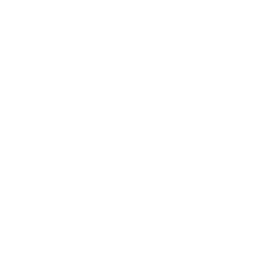
\includegraphics[scale=1]{assets/branding/opa0}
    \vspace{-5.75cm}\\
    {\adjustbox{scale=1.65}{\color{TealDarkCyan}\;II.\;When Decoding Is Easy}}
    \vspace{.25cm}
    \begin{minipage}{.78\textwidth}
      \scriptsize\color{Ink}
      \textbf{Big picture.}\;
      Algebraic structure turns the syndrome from a clue into an address: it names the error exactly.\\[.2cm]
      \textbf{Details to watch.}\;
      generator matrix, parity-check matrix, syndrome, Hamming bound, perfect code, cyclic ideal, quasi-cyclic hint.
    \end{minipage}
    {\ }\vspace{2.1cm}\\
    \bigskip
  \end{center}
\end{frame}

%=== A. LINEAR CODES ===

%--- Linear code definition ---
\begin{frame}{\textbf{II. When Decoding Is Easy}}{Linear Codes}
\small
\defbox[{Linear $[n,k,d]_q$ Code}]{
A \textbf{linear code} is a $k$-dimensional subspace $\code\le\F_q^n$ with minimum Hamming distance $d$.
Its elements are \textbf{codewords}.
}
\begin{columns}[T,onlytextwidth]
\begin{column}{.52\textwidth}
\defbox[Generator matrix]{
$\mat G\in\F_q^{k\times n}$: rows form a basis of $\code$.
Encoding: $\vect m \mapsto \vect c = \vect m\mat G$.
}
\defbox[Parity-check matrix]{
$\mat H\in\F_q^{(n-k)\times n}$: $\code = \ker(\mat H)$.
Check: $\vect c\in\code \Leftrightarrow \mat H\vect c^T = \vect 0$.
}
\end{column}
\begin{column}{.44\textwidth}
\textcolor{TealDarkCyan}{\textbf{Parameters}}
\begin{itemize}
  \item Rate $R=k/n$ (information density)
  \item Redundancy $r=n-k$ (check symbols)
  \item Distance $d$ (error budget)
\end{itemize}
\bigskip
\textcolor{TealDarkCyan}{\textbf{Error capability}}
\[
  t = \left\lfloor\frac{d-1}{2}\right\rfloor\;\text{errors corrected}
\]
\end{column}
\end{columns}
\end{frame}

%--- Systematic form + tikz ---
\begin{frame}{\textbf{II. When Decoding Is Easy}}{Systematic Form and Encoding}
\small
\defbox[Systematic form]{
$\mat G = [\mat I_k \mid \mat P]$: first $k$ coordinates carry the message; last $n-k$ are parity.
}
\begin{center}
\begin{tikzpicture}[x=1cm,y=1cm]
  \node[process] (msg) at (-4.55,0) {$\vect m$\\[-1pt]\scriptsize message};
  \foreach \i/\b in {1/1,2/0,3/1,4/1}{
    \node[bit teal,right={-0.01cm of msg},xshift={0.45*\i cm-0.2cm}]
      at (-5.8+0.05*\i,-1) {$\b$};
  }
  \node[process blue,minimum width=2.35cm,minimum height=1.48cm] (G) at (0,0)
    {\large $\mat G=[\mat I_k\mid \mat P]$};
  \node[process amber] (code) at (4.45,0) {$\vect c=\vect m\mat G$\\[-1pt]\scriptsize codeword};
  \foreach \i/\b in {1/1,2/0,3/1,4/1,5/0,6/0,7/1}{
    \ifnum\i<5
      \node[bit teal]  at (2.6+0.46*\i,-1) {$\b$};
    \else
      \node[bit amber] at (2.6+0.46*\i,-1) {$\b$};
    \fi
  }
  \draw[decorate,decoration={brace,amplitude=4pt},TealDarkCyan!75,line width=0.7pt]
    (4.66,-1.35) -- (2.86,-1.35) node[midway,below=0.12cm,tiny label]{message};
  \draw[decorate,decoration={brace,amplitude=4pt},AmberCode!85,line width=0.7pt]
    (6.06,-1.35) -- (4.66,-1.35) node[midway,below=0.12cm,tiny label]{parity};
  \draw[flow]      (msg) -- (G)    node[midway,above=0.12cm,tiny label]{linear map};
  \draw[flow blue] (G)   -- (code) node[midway,above=0.12cm,tiny label]{redundancy};
\end{tikzpicture}
\end{center}
\textbf{Example.}\; For the $[7,4,3]_2$ Hamming code with $\vect m=(1,0,1,1)$:
$\vect c = \vect m\mat G = (1,0,1,1,0,1,0)$.
\end{frame}

%--- Parity-check matrix + syndrome ---
\begin{frame}{\textbf{II. When Decoding Is Easy}}{Syndrome: The Error Fingerprint}
\small
\defbox[Syndrome]{
For received $\vect y = \vect c + \vect e$,
\[
  \vect s = \mat H\vect y^T = \underbrace{\mat H\vect c^T}_{=\,\vect 0} + \mat H\vect e^T = \mat H\vect e^T.
\]
The syndrome depends \emph{only on the error}, not on which codeword was sent.
}
\[
  \mat H = \begin{bmatrix}
    0&1&1&1&1&0&0\\
    1&0&1&1&0&1&0\\
    1&1&0&1&0&0&1
  \end{bmatrix}
  \xrightarrow{\;\mat H\vect e^T\;}
  \vect s = \begin{pmatrix}1\\0\\0\end{pmatrix}
\]
\begin{itemize}
  \item $\vect s = \vect 0$ iff $\vect y\in\code$ (no detectable error).
  \item Every nonzero $\vect s$ identifies the coset $\vect e + \code$.
  \item \textbf{Decoding} = find the minimum-weight $\vect e$ with $\mat H\vect e^T = \vect s$.
\end{itemize}
\end{frame}

%--- Distance theorem + packing ---
\begin{frame}{\textbf{II. When Decoding Is Easy}}{Error Correction and the Hamming Bound}
\small
\begin{columns}[T,onlytextwidth]
\begin{column}{.50\textwidth}
\thmbox[Distance theorem]{
A code of distance $d$ corrects every error of weight $\le t = \lfloor(d-1)/2\rfloor$
and detects every error of weight $\le d-1$.
}
\vspace{.4em}
\thmbox[Hamming bound]{
$\displaystyle q^k\sum_{i=0}^t\binom{n}{i}(q-1)^i \le q^n.$
}
\defbox[Perfect code]{
Equality in the Hamming bound: correction balls of radius $t$ tile $\F_q^n$ with \emph{no gaps and no overlap}.
}
\end{column}
\begin{column}{.46\textwidth}
\begin{center}
\begin{tikzpicture}[scale=.88]
  \fill[TealDarkCyan!6] (-2.8,-2.3) rectangle (2.8,2.3);
  \node[font=\tiny,TealDarkCyan!60] at (2.2,2.0) {$\F_2^n$};
  \fill[AccentCyan!25] (-1.4, 0.9) circle (.75);
  \fill[TealDarkCyan]  (-1.4, 0.9) circle (3pt) node[above=3pt,font=\tiny]{$c_1$};
  \fill[AccentCyan!25] ( 1.3, 0.9) circle (.75);
  \fill[TealDarkCyan]  ( 1.3, 0.9) circle (3pt) node[above=3pt,font=\tiny]{$c_2$};
  \fill[AccentCyan!25] ( 0.0,-1.1) circle (.75);
  \fill[TealDarkCyan]  ( 0.0,-1.1) circle (3pt) node[above=3pt,font=\tiny]{$c_3$};
  \node[font=\tiny,AccentCyan!70!TealDarkCyan] at (-2.3,-0.6) {balls};
  \node[font=\tiny,AccentCyan!70!TealDarkCyan] at (-2.3,-0.9) {radius $t$};
  \draw[dashed,TealDarkCyan!50] (-2.8,0)--(2.8,0);
  \node[font=\tiny,TealDarkCyan!50] at (2.1,-.2) {no overlap};
\end{tikzpicture}
\end{center}
\end{column}
\end{columns}
\end{frame}

%=== B. HAMMING CODES ===

%--- Historical motivation ---
\begin{frame}{\textbf{II. When Decoding Is Easy}}{Hamming (1950): The Original Insight}
\small
\begin{columns}[T,onlytextwidth]
\begin{column}{.54\textwidth}
Richard Hamming at Bell Labs in 1947: punched-card overnight jobs crashed on \emph{single-bit errors}.

\medskip
\textbf{His question:} ``If the machine can \emph{detect} an error, why can't it \emph{fix} it?''

\medskip
\defbox[Hamming's key idea]{
Add redundant parity bits so that:
\begin{itemize}
  \item the syndrome names the \textbf{exact error position}, and
  \item \textbf{no syndrome is wasted} — every nonzero syndrome maps to a unique error.
\end{itemize}
}
One error at position $i$, or no error: $n+1$ cases, $2^r$ syndromes.
\[
  n+1=2^r \;\Longrightarrow\; n=2^r-1.
\]
\end{column}
\begin{column}{.43\textwidth}
\begin{tikzpicture}[scale=.88]
  \node[font=\small\bfseries,TealDarkCyan] at (1.5,4.0) {Syndrome $\to$ action};
  \draw[TealDarkCyan,thick] (0,3.65)--(3.0,3.65);
  \node[draw=TealDarkCyan!40,rounded corners=3pt,fill=TealDarkCyan!8,
        minimum width=2.8cm,minimum height=0.38cm,font=\scriptsize]
    at (1.5,3.25) {$000$ $\to$ no error};
  \foreach \i/\bits in {1/001, 2/010, 3/011, 4/100, 5/101, 6/110, 7/111}{
    \pgfmathsetmacro{\yy}{3.25-\i*0.42}
    \node[draw=AccentCyan!60,rounded corners=3pt,fill=AccentCyan!10,
          minimum width=2.8cm,minimum height=0.38cm,font=\scriptsize]
      at (1.5,\yy) {$\bits$ $\to$ flip bit $\i$};
  }
\end{tikzpicture}
\end{column}
\end{columns}
\end{frame}

%--- Hamming code definition ---
\begin{frame}{\textbf{II. When Decoding Is Easy}}{The Binary Hamming Code}
\small
\defbox[Binary Hamming matrix $\mat H_r$]{
$\mat H_r$ is the $r\times(2^r-1)$ matrix whose columns are \emph{all nonzero binary vectors} of length $r$.
}
\[
  \mat H_3=\begin{bmatrix}1&0&1&0&1&0&1\\0&1&1&0&0&1&1\\0&0&0&1&1&1&1\end{bmatrix}.
\]
\defbox[Binary Hamming code]{
$\operatorname{Ham}(r,2)=\ker(\mat H_r)$, with parameters $[2^r-1,\;2^r-1-r,\;3]_2$.
}
\begin{columns}[T,onlytextwidth]
\begin{column}{.50\textwidth}
\begin{itemize}
  \item Every nonzero syndrome identifies a unique column of $\mat H_r$.
  \item The column label is the binary address of the error.
  \item Corrects exactly one error; detects exactly two.
\end{itemize}
\end{column}
\begin{column}{.46\textwidth}
\thmbox[Perfect]{
$2^k(1+n) = 2^{2^r-1}$ — the correction balls tile all of $\F_2^n$.
}
\end{column}
\end{columns}
\end{frame}

%--- Perfect tiling ---
\begin{frame}{\textbf{II. When Decoding Is Easy}}{Perfect Tiling: Why Hamming Codes Are Special}
\small
\begin{columns}[T,onlytextwidth]
\begin{column}{.47\textwidth}
For $[3,1,3]_2$ in $\F_2^3$: two correction balls of radius 1
\textbf{tile the cube exactly} — no overlap, no gap.
\begin{center}
\begin{tikzpicture}[scale=.78]
  \draw[gray!35,thick] (0,0)--(2,0); \draw[gray!35,thick] (0,0)--(1,.9);
  \draw[gray!35,thick] (0,0)--(.5,1.6); \draw[gray!35,thick] (2,0)--(3,.9);
  \draw[gray!35,thick] (2,0)--(2.5,1.6); \draw[gray!35,thick] (1,.9)--(3,.9);
  \draw[gray!35,thick] (1,.9)--(1.5,2.5); \draw[gray!35,thick] (.5,1.6)--(2.5,1.6);
  \draw[gray!35,thick] (.5,1.6)--(1.5,2.5); \draw[gray!35,thick] (3,.9)--(3.5,2.5);
  \draw[gray!35,thick] (2.5,1.6)--(3.5,2.5); \draw[gray!35,thick] (1.5,2.5)--(3.5,2.5);
  \foreach \x/\y/\col in {0/0/TealDarkCyan, 2/0/TealDarkCyan,
                           1/.9/TealDarkCyan, .5/1.6/TealDarkCyan}{
    \node[circle,draw=\col,fill=\col!20,minimum size=.60cm,font=\tiny\bfseries]
      at (\x,\y) {};
  }
  \foreach \x/\y/\s in {0/0/$000$, 2/0/$100$, 1/.9/$010$, .5/1.6/$001$}{
    \node[font=\tiny] at (\x,\y) {\s};
  }
  \foreach \x/\y/\col in {3.5/2.5/AccentCyan, 1.5/2.5/AccentCyan,
                           2.5/1.6/AccentCyan, 3/.9/AccentCyan}{
    \node[circle,draw=\col,fill=\col!22,minimum size=.60cm,font=\tiny\bfseries]
      at (\x,\y) {};
  }
  \foreach \x/\y/\s in {3.5/2.5/$111$, 1.5/2.5/$011$, 2.5/1.6/$101$, 3/.9/$110$}{
    \node[font=\tiny] at (\x,\y) {\s};
  }
  \node[below=3pt,font=\tiny,TealDarkCyan] at (0,0) {\textbf{c=000}};
  \node[above=3pt,font=\tiny,AccentCyan]   at (3.5,2.5) {\textbf{c=111}};
\end{tikzpicture}
\end{center}
\end{column}
\begin{column}{.50\textwidth}
\textcolor{TealDarkCyan}{\textbf{Why ``perfect''?}}
\begin{itemize}
  \item Each ball: 1 codeword + 3 distance-1 neighbours = 4 words
  \item Two balls cover all $2^3=8$ points; $2\times4=8$ ✓
  \item For $\operatorname{Ham}(r,2)$: $2^{2^r-1-r}\times 2^r = 2^{2^r-1}$ ✓
\end{itemize}

\medskip
\defbox[The decoder is one table look-up]{
Syndrome $\vect s\ne\vect 0$: find the unique column $i$ of $\mat H_r$ equal to $\vect s$.
Flip bit $i$.  Time: $O(1)$.
}

\medskip
No other linear perfect single-error-correcting code exists (apart from trivial cases).
\end{column}
\end{columns}
\end{frame}

%--- Encoding + syndrome walkthrough ---
\begin{frame}{\textbf{II. When Decoding Is Easy}}{Encoding and Correction: The Full Picture}
\small
\begin{center}
\begin{tikzpicture}[
  box/.style={draw=TealDarkCyan,thick,rounded corners=4pt,
              minimum width=2.0cm,minimum height=0.65cm,
              fill=TealDarkCyan!10,font=\scriptsize,align=center},
  earr/.style={-Stealth,thick,AccentCyan,dashed}
]
  \node[box] (msg)  at (0,0)   {Message\\$m=(1,0,1,1)$};
  \node[box] (enc)  at (3,0)   {Encoder\\$c=mG$};
  \node[box] (cw)   at (6,0)   {Codeword\\$c=(1,0,1,1,0,1,0)$};
  \node[box,fill=AccentCyan!12,draw=AccentCyan] (ch) at (9,0)
    {Channel\\flip bit 5};
  \node[box,fill=AccentCyan!8,draw=AccentCyan]  (rv)  at (9,-1.5)
    {Received\\$v=(1,0,1,1,\mathbf{1},1,0)$};
  \node[box] (syn)  at (6,-1.5) {Syndrome\\$s=(1,0,1)^T$};
  \node[box] (lkp)  at (3,-1.5) {Look up\\col 5 of $H$};
  \node[box] (fix)  at (0,-1.5) {Correct\\$\hat c=c$ \checkmark};
  \draw[-Stealth,thick,TealDarkCyan] (msg)--(enc);
  \draw[-Stealth,thick,TealDarkCyan] (enc)--(cw);
  \draw[-Stealth,thick,TealDarkCyan] (cw)--(ch);
  \draw[earr] (ch)--(rv);
  \draw[-Stealth,thick,TealDarkCyan] (rv)--(syn);
  \draw[-Stealth,thick,TealDarkCyan] (syn)--(lkp);
  \draw[-Stealth,thick,TealDarkCyan] (lkp)--(fix);
  \node[above=2pt,font=\tiny,TealDarkCyan] at (1.5,0)  {$mG$};
  \node[above=2pt,font=\tiny,AccentCyan]   at (9,-.75) {noise};
  \node[above=2pt,font=\tiny,TealDarkCyan] at (7.5,-1.5){$Hv^T$};
\end{tikzpicture}
\end{center}
\begin{columns}[T,onlytextwidth]
\begin{column}{.50\textwidth}
\begin{itemize}
  \item Syndrome $(1,0,1)^T$ = column 5 of $\mat H_3$
  \item Flip bit 5 to recover $c$ ✓
  \item The decoder \emph{never} needs to know $m$
\end{itemize}
\end{column}
\begin{column}{.46\textwidth}
\textcolor{TealDarkCyan}{\textbf{This is why Hamming codes work:}}
the syndrome is literally the binary address of the error.
No search, no iteration.
\end{column}
\end{columns}
\end{frame}

%--- The Fano plane ---
\begin{frame}{\textbf{II. When Decoding Is Easy}}{Geometry Behind the Code: The Fano Plane}
\small
\begin{columns}[T,onlytextwidth]
\begin{column}{.44\textwidth}
\begin{center}
\begin{tikzpicture}[scale=.85]
  \draw[TealDarkCyan,thick] (0,2) -- (-1.73,-1);
  \draw[TealDarkCyan,thick] (0,2) -- (1.73,-1);
  \draw[TealDarkCyan,thick] (-1.73,-1) -- (1.73,-1);
  \draw[AccentCyan,thick]  (0,2) -- (0,-1);
  \draw[AccentCyan,thick]  (-1.73,-1) -- (.865,.5);
  \draw[AccentCyan,thick]  (-.865,.5) -- (1.73,-1);
  \draw[TealDarkCyan!55,thick] (0,0) circle (1.0);
  \fill[TealDarkCyan] (0,2)     circle (3.5pt);
  \node[above=3pt,font=\scriptsize,TealDarkCyan] at (0,2) {$1$};
  \fill[TealDarkCyan] (-1.73,-1)circle (3.5pt);
  \node[left=3pt,font=\scriptsize,TealDarkCyan]  at (-1.73,-1){$2$};
  \fill[TealDarkCyan] (1.73,-1) circle (3.5pt);
  \node[right=3pt,font=\scriptsize,TealDarkCyan] at (1.73,-1) {$4$};
  \fill[AccentCyan] (-.865,.5)  circle (3.5pt);
  \node[left=3pt,font=\scriptsize,AccentCyan]    at (-.865,.5){$3$};
  \fill[AccentCyan] (.865,.5)   circle (3.5pt);
  \node[right=3pt,font=\scriptsize,AccentCyan]   at (.865,.5) {$5$};
  \fill[AccentCyan] (0,-1)      circle (3.5pt);
  \node[below=3pt,font=\scriptsize,AccentCyan]   at (0,-1)    {$6$};
  \fill[TealDarkCyan!70] (0,0)  circle (3.5pt);
  \node[right=4pt,font=\scriptsize,TealDarkCyan] at (0,0)     {$7$};
\end{tikzpicture}
\end{center}
\end{column}
\begin{column}{.53\textwidth}
\textcolor{TealDarkCyan}{\textbf{The 7 lines $\leftrightarrow$ 7 weight-3 codewords:}}
\smallskip
\begin{tabular}{c|c}
  Line & Columns sum to $\vect 0$ \\\hline
  \rowcolor{TealDarkCyan!8} $\{1,2,3\}$ & $100\oplus010=110$ \\
  $\{1,4,5\}$ & $100\oplus001=101$ \\
  \rowcolor{TealDarkCyan!8} $\{2,4,6\}$ & $010\oplus001=011$ \\
  $\{1,6,7\}$ & $100\oplus011=111$ \\
  \rowcolor{TealDarkCyan!8} $\{2,5,7\}$ & $010\oplus101=111$ \\
  $\{3,4,7\}$ & $110\oplus001=111$ \\
  \rowcolor{TealDarkCyan!8} $\{3,5,6\}$ & $110\oplus101=011$ \\
\end{tabular}
\bigskip

$d=3$ because the smallest Fano line has 3 points.
Algebraic structure = geometric minimum.
\end{column}
\end{columns}
\end{frame}

%=== C. CYCLIC CODES AND QUASI-CYCLIC ===

%--- Cyclic shift = polynomial multiplication ---
\begin{frame}{\textbf{II. When Decoding Is Easy}}{Cyclic Codes: Shift Symmetry}
\small
\defbox[Cyclic code]{
$\code\le\F_q^n$ is cyclic if $(c_0,\ldots,c_{n-1})\in\code \Rightarrow (c_{n-1},c_0,\ldots,c_{n-2})\in\code$.
}
Under the identification $(c_0,\ldots,c_{n-1})\leftrightarrow c(X)=c_0+c_1X+\cdots+c_{n-1}X^{n-1}$
in $R_n=\F_q[X]/(X^n-1)$:
\begin{itemize}
  \item cyclic shift = multiply by $X$ in $R_n$
  \item a cyclic code = an \textbf{ideal} in $R_n$ = $\ideal{g(X)}$ for a unique monic divisor $g(X)\mid X^n-1$
\end{itemize}
\begin{columns}[T,onlytextwidth]
\begin{column}{.50\textwidth}
\defbox[BCH bound]{
Prescribe $\delta-1$ consecutive roots $\alpha^b,\ldots,\alpha^{b+\delta-2}$ of $g(X)$.
Then $d\ge\delta$.
}
\end{column}
\begin{column}{.46\textwidth}
\textcolor{TealDarkCyan}{\textbf{Hardware bonus}}

Division by $g(X)$ computes via a shift register with $n-k$ flip-flops.
Encoding and syndrome computation run at wire speed.
\end{column}
\end{columns}
\textbf{Example.}\; $X^7-1=(X+1)(X^3+X+1)(X^3+X^2+1)$ over $\F_2$.
Taking $g=X^3+X+1$ gives the cyclic $[7,4,3]_2$ Hamming code.
\end{frame}

%--- Decoding summary for algebraic codes ---
\begin{frame}{\textbf{II. When Decoding Is Easy}}{Why Algebraic Structure Makes Decoding Easy}
\small
\begin{center}
\renewcommand{\arraystretch}{1.28}
\begin{tabular}{p{.22\textwidth}p{.26\textwidth}p{.40\textwidth}}
\toprule
Code family & Structure & Decoding mechanism \\
\midrule
Hamming $[2^r-1,*,3]_2$ & Projective parity checks & Syndrome = binary address; $O(1)$ table look-up \\
Cyclic (BCH, RS) & Ideal in $\F_q[X]/(X^n-1)$ & Root syndromes + Berlekamp--Massey; $O(n^2)$ \\
Reed--Solomon & Evaluation code; MDS & Welch--Berlekamp; $O(n^2)$ \\
LDPC / Turbo & Sparse Tanner graph & Belief propagation; near-linear \\
\bottomrule
\end{tabular}
\end{center}
\bigskip
\textbf{The pattern.}\;
Every efficient decoder exploits a specific algebraic invariant.
Projective geometry gives Hamming its $O(1)$ decoder.
Polynomial roots give BCH and RS their syndromes.
\medskip
\begin{alertblock}{}
\centering
Remove the algebraic structure \textbf{$\rightarrow$} no formula \textbf{$\rightarrow$} exponential search.
\end{alertblock}
\end{frame}

%--- Quasi-cyclic hint and transition ---
\begin{frame}{\textbf{II. When Decoding Is Easy}}{Quasi-Cyclic Codes: A Bridge to Cryptography}
\small
\defbox[Quasi-cyclic code of index $\ell$]{
$\code\subseteq\F_q^n$ ($n=\ell m$) is \textbf{quasi-cyclic} if it is invariant under cyclic shift by $\ell$ positions.
Generator matrices are built from $\ell\times\ell$ \textbf{circulant blocks} — each block described by one polynomial in $R_m=\F_q[X]/(X^m-1)$.
}
\begin{columns}[T,onlytextwidth]
\begin{column}{.52\textwidth}
\textcolor{TealDarkCyan}{\textbf{Why QC codes matter in cryptography}}
\begin{itemize}
  \item Entire parity-check matrix compressed from $O(n^2)$ to $O(n)$ bits.
  \item Arithmetic in $R_m$: polynomial multiplication, inversion.
  \item Random-looking but algebraically structured.
  \item Retains hardness of decoding — but now opens new attack surfaces.
\end{itemize}
\end{column}
\begin{column}{.44\textwidth}
\begin{center}
\begin{tikzpicture}[node distance=.5cm,scale=.80,transform shape]
  \node[process]              (cyc)  {cyclic code\\ideal in $R_n$};
  \node[process blue,below=of cyc]  (qc)   {quasi-cyclic\\$\ell$ circulant blocks};
  \node[process amber,below=of qc]  (hard) {QCSD\\hard search problem};
  \node[process red,below=of hard]  (pqc)  {BIKE/HQC\\PQC system};
  \draw[flow]       (cyc) -- (qc);
  \draw[flow blue]  (qc)  -- (hard);
  \draw[flow amber] (hard)-- (pqc);
\end{tikzpicture}
\end{center}
\end{column}
\end{columns}
\medskip
\textbf{Coming up:} We now ask what happens when we \emph{remove} algebraic structure entirely and face a random parity-check matrix.
\end{frame}
